{$\space$\par}
\vspace{0.5cm}
\justifying
\section*{{\bfseries \LARGE Questão 1 -} {\bfseries \large  Represente cada aluno por uma Face de Chernoff. A partir delas, você julga que há alunos que apresentem um histórico no ENEM e CRA do primeiro período similar entre si? Ou não?}}

\vspace{0.2cm}

\textcolor{red}{Um bom método para exploração e classificação é o de Faces de Chernoff que utiliza característica físicas para exemplificar o quão similar os dados são no espaço de seus parâmetros. Duas faces similares indicam pontos que estão em uma região próxima no espaço dos parâmetros. Esse método facilita para humanos avaliarem similaridades nos dados e então poder trabalhar em cima dessa análise inicial. Para isso usei a função \texttt{faces} considerando todas as colunas da amostra de alunos da astronomia, exceto seus nomes e o ano da turma, já que não são relevantes ao olhar para a nota do Enem e o CRA.}

\vspace{0.2cm}

\begin{lstlisting}
    install.packages('TeachingDemos')
    library(TeachingDemos)

    astro = read.table('/content/ENEM_Astro.csv', sep=',', header=T)
    
    options(repr.plot.width=14,repr.plot.height=12)
    # Usando todas colunas, exceto o nome para criar as faces
    faces(astro[, 2:7], labels = astro$Nome)
\end{lstlisting}


\begin{figure}[h]
    \centering
    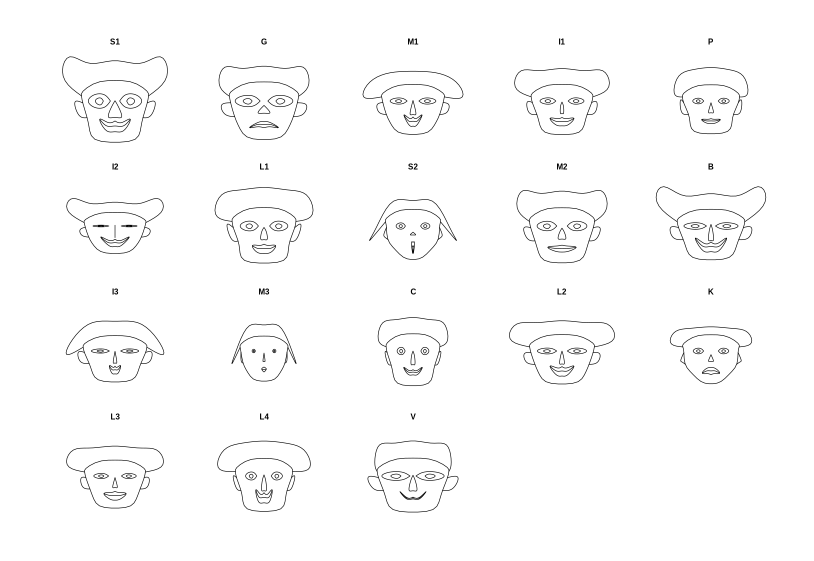
\includegraphics[width=0.8\linewidth]{Figuras/Faces.png}
    \caption{Resultado ao aplicar o método de faces de Chernoff na amostra de alunos da astronomia.}
    \label{faces}
\end{figure}

\textcolor{red}{O resultado pode ser visto na imagem \ref{faces}, onde é possível dizer que de fato há alunos similares nesse espaço de parâmetros. Os principais grupo que percebi foi o de: (S1, B), (S2, M3) e (L1, L2, L3) como indicado na imagem.}